\pdfoutput=1
\documentclass[10pt]{beamer}

%STANDARD PREAMBLE
%https://tex.stackexchange.com/questions/68821/is-it-possible-to-create-a-latex-preamble-header
\usepackage{../../rsrc/beamer_preamble}

% RANDOM VARIABLE
\newcommand{\x}{X}
\newcommand{\y}{Y}


% CREATE DIFFERENT VERSIONS DEPENDING ON THE AUDIENCE
% Reference: https://tex.stackexchange.com/questions/290102/how-do-i-skip-slides-in-beamer
% Audiences: {researchers, students}
\usepackage[
    audience=students
    ]{beameraudience}
    
\title{Independence Properties \\ of Directed Probabilistic Graphical Models}

\begin{document}

\maketitle

\begin{frame}{Table of contents}
  \setbeamertemplate{section in toc}[sections numbered]
  \tableofcontents[hideallsubsections]
\end{frame}

\section{Motivation}

\justfor{students}{
\begin{frame}{Introductory Question}

\bf{Claim:}  Buying margarine is unethical.  \pause

\bf{Argument:}
\begin{center}
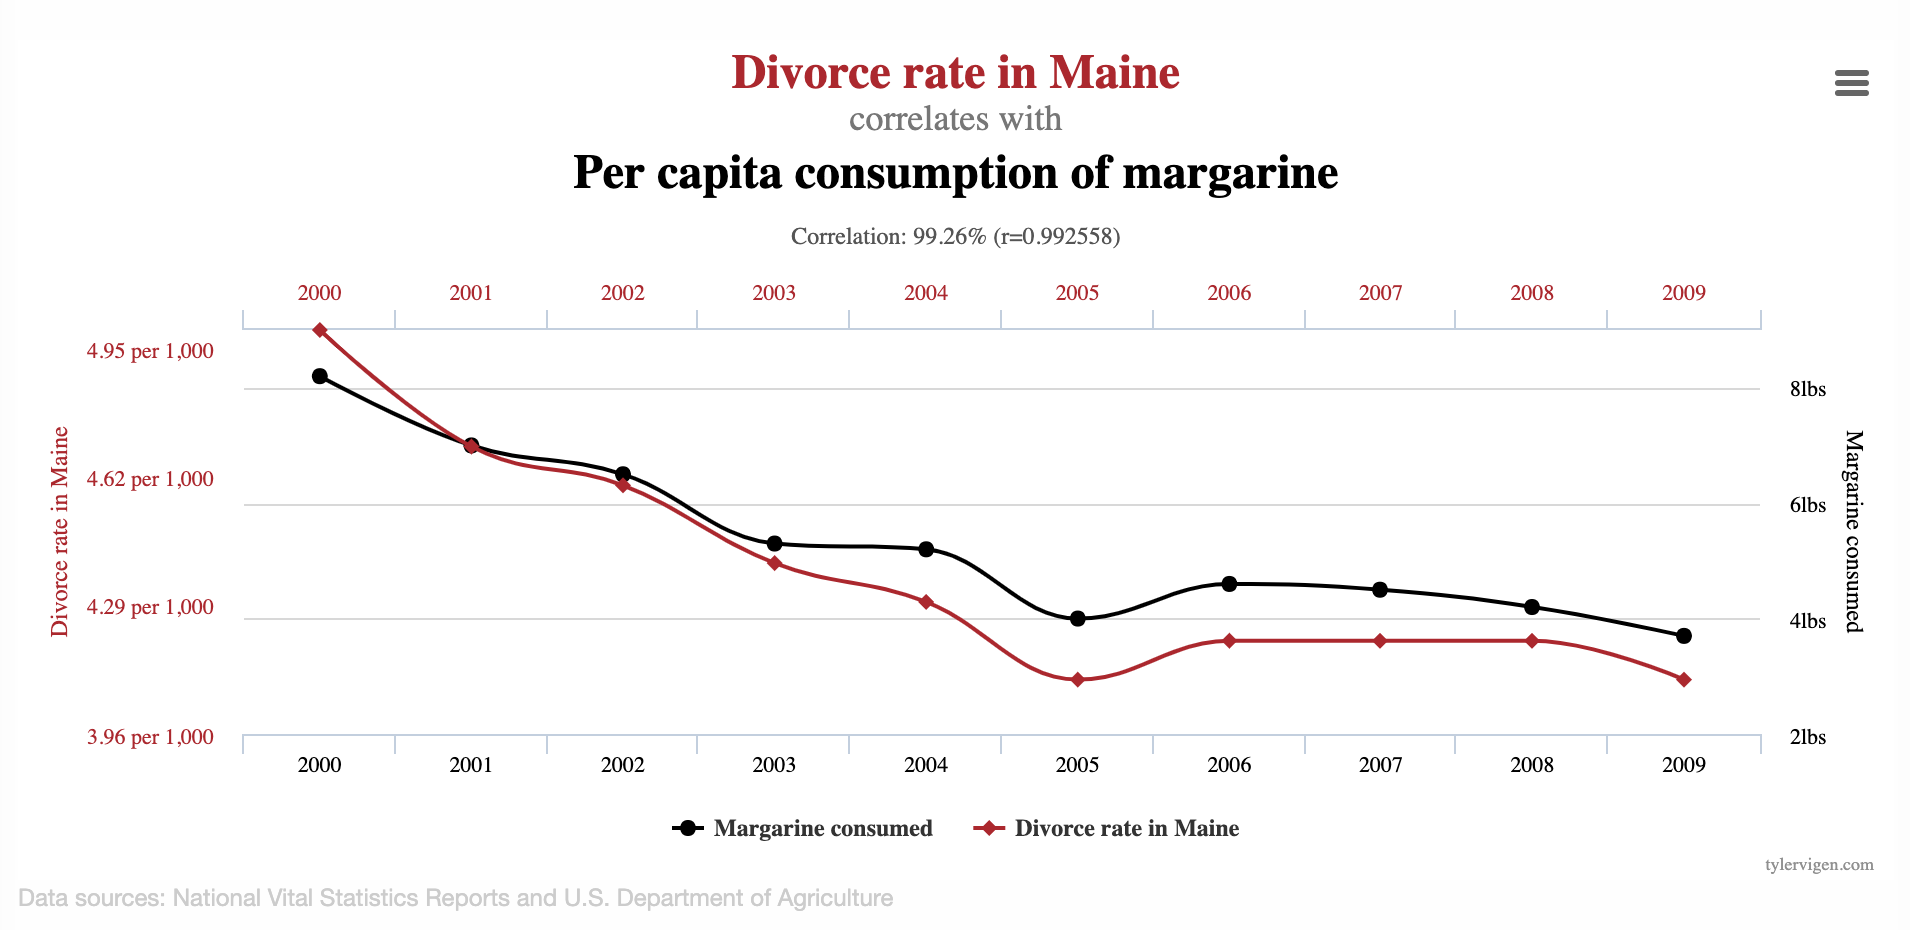
\includegraphics[width=\textwidth]{images/divorce_and_margarine}
\end{center}
\pause 

\bf{Q:}  What are the problems with this argument?
% SAY: 1) p-hacking (note they only pick Maine)
% 2) corr does not imply causation 
% 2a) In particular, a third-variable problem.  What do you think the third variable is?
\end{frame}



\begin{frame}{Marginal vs. Conditional Independence}

\begin{center}
\textbf{The``third variable" problem}
\end{center}

\vfill \vfill
\begin{columns}[onlytextwidth,t]
 \begin{column}{0.5\textwidth}
  \centering
   % \textbf{Common parent} \\[.3cm]
		  \scalebox{0.7}{
		  \tikz{ %
		    \node[latent] (y) at (0,0) {$time$} ; %
		    \node[latent] (x) at (-2,-4) {$divorces$} ; %
		    \node[latent] (z) at (2,-4) {$margarine$} ; %
		 \edge{y}{x};
		 \edge{y}{z};
		 }
	}\\[.3cm] 
	\[ \text{divorces} \not\indep \text{margarine} \]
    \end{column}
    
    
     \begin{column}{0.33\textwidth}
  \centering
    %\textbf{Common parent} \\[.3cm]
		  \scalebox{0.7}{
		  \tikz{ %
		    \node[obs] (y) at (0,0) {$time$} ; %
		    \node[latent] (x) at (-2,-4) {$divorces$} ; %
		    \node[latent] (z) at (2,-4) {$margarine$} ; %
		 \edge{y}{x};
		 \edge{y}{z};
		 }
	}\\[.3cm] 
	\[ \text{divorces} \indep \text{margarine} \cond \text{time} \]
    \end{column}

\end{columns}
    
\end{frame}


\begin{frame}{Marginal vs. Conditional Independence}

\begin{columns}[onlytextwidth,t]
 \begin{column}{0.5\textwidth}
  \centering
    \textbf{Common parent} \\[.3cm]
		  \scalebox{0.7}{
		  \tikz{ %
		    \node[latent] (y) at (0,0) {$Y$} ; %
		    \node[latent] (x) at (-2,-4) {$X$} ; %
		    \node[latent] (z) at (2,-4) {$Z$} ; %
		 \edge{y}{x};
		 \edge{y}{z};
		 }
	}\\[.3cm] 
	\[ Z \not\indep X \]
    \end{column}
    
    
     \begin{column}{0.33\textwidth}
  \centering
    \textbf{Common parent} \\[.3cm]
		  \scalebox{0.7}{
		  \tikz{ %
		    \node[obs] (y) at (0,0) {$Y$} ; %
		    \node[latent] (x) at (-2,-4) {$X$} ; %
		    \node[latent] (z) at (2,-4) {$Z$} ; %
		 \edge{y}{x};
		 \edge{y}{z};
		 }
	}\\[.3cm] 
	\[ Z \indep X \cond Y \]
    \end{column}

\end{columns}

\end{frame}


}
% Say: They are marginally dependent but conditionally independent


\begin{frame}{Motivation}
\scriptsize
Consider  a Bayesian Hidden Markov Model \\

You may see statements like: \textit{The future is independent of the past given the current hidden state.}

\pause
\begin{itemize}
\item How can we know this?
\pause 
\item More generally:  How can we easily answer queries about \tiny (conditional \textit{or} marginal) \scriptsize independence ?
\end{itemize}

\pause  
\begin{block}{Joint Distribution}
\tiny Notating transition matrix $\pi$,  emissions parameters $\theta$. hidden states $X$, and observations $Y$, and suppressing hyperparameters, we have \scriptsize  

\[  \underset{joint \, density}{p(\pi, \theta, X, Y)} = \explaintermbrace{prior}{p(\pi) \, p(\theta)} \quad 
\explaintermbrace{(complete data) likelihood}{ p(X_0) \; \ds\prod_{t=1}^T p_\pi(X_t \cond X_{t-1})  \; p_\theta (Y_t \cond X_t)} \]
\end{block}


\pause 
%We can make headway by representing the model as a \bf{probabilistic graphical model.}

\begin{block}{Representation as a \textit{probabilistic graphical model}}
\begin{center}
  \scalebox{0.5}{
  \tikz{ %
    \node[latent] (pi) {$\pi_k$} ; %
    \node[latent, below=of pi] (theta) {$\theta_k$} ; %
    \node[const, left=of pi] (alpha) {$\alpha$}; %
     \node[const, left=of theta] (H) {$H$}; %
 \plate[inner sep=0.25cm, xshift=0cm, yshift=0cm] {plate1} {(pi) (theta)} {$K$}; %
     \node[obs, right=of pi](x0){$\x_0$}; %
     \node[latent, right=of x0](x1){$\x_1$}; %
     \node[latent, right=of x1](x2){$\x_2$};%
     \node[const, right=of x2](ellipses){$\; \+\ldots \;$}; %
     \node[latent, right=of ellipses](xT){$\x_T$}; %
     \draw [->] (pi) to [out=30, in=150] (x1);
     \draw [->] (pi) to [out=30, in=150] (x2);
     \draw [->] (pi) to [out=30, in=150] (xT);
     \node[obs, below=of x1](y1){$\y_1$}; %
     \node[obs, right=of y1](y2){$\y_2$};%
     \node[const, right=of y2](yellipses){$\; \+\ldots \;$}; %
     \node[obs, right=of yellipses](yT){$\y_T$}; %
     \draw [->] (theta) to [out=30, in=150] (y1);
     \draw [->] (theta) to [out=30, in=150] (y2);
     \draw [->] (theta) to [out=30, in=150] (yT);
 \edge{alpha}{pi} ;
 \edge{H}{theta} ;
 \edge{x0}{x1};
 \edge{x1}{x2};
  \edge{x2}{ellipses};
  \edge{ellipses}{xT};
  \edge{x1}{y1};
   \edge{x2}{y2};
  \edge{xT}{yT};
  }
 }
\end{center}
\end{block}

\end{frame}




\section{Directed Probabilistic  Graphical Models }
\begin{frame}{Joint distributions}
The starting point for a directed probabilistic graphical model is a particular factorization of a joint density:

\begin{equation}
\label{eqn:joint_factorization}
 p(\x_1, ..., \x_n) = \ds\prod_{i=1}^n p(\x_i \cond \pi_i ) 
\end{equation}

where the conditioning set $\pi_i$ is referred to as the \alert{parents} of  variable $i$. \\

\justfor{students}{
	
	\tiny ( In the intro example, who are the parents of margarine? \pause 
	In the HMM example, who are the parents of the hidden state $x_t$?  Of the observation $y_t$? ) \normalsize \pause

} 
\eqref{eqn:joint_factorization} simplifies the factorizations which are \textit{always} true, by the chain rule of probability:

\[ p(\x_1, ..., \x_n) = \ds\prod_{i=1}^n p(\x_i \cond \x_1, .., \x_{i-1} ) \]


\justfor{researchers}{
	\pause
	\vfill \vfill

	\tiny In other words, \eqref{eqn:joint_factorization} restricts our consideration to a certain subset of joint probability distributions.  \\
	
	\pause
	\tiny Consider, e.g., the structure imposed in Bayesian models by independent priors or conditionally i.i.d likelihoods.  \normalsize
}

\end{frame}

%The problem is that it is not clear in advance that the arbitrary collection of conditionals given in \eqref{eqn:joint_factorization} is internally consistent, and are indeed the conditionals for the provided joint.  Luckily, there is a theorem (not proven here) which guarantees this to be true.\footnote{This may be demonstrated in Chapter 3 of \cite{koller}; I'm not sure.}

\begin{frame}{Directed probabilistic graphical models} 
\footnotesize 
Once we have specified our desired factorization via \eqref{eqn:joint_factorization}, we can identify it with a directed acyclic graph (DAG) $\mathcal{G} = (E,V)$ by:
\begin{itemize}
\item identifying each random variable with a node \pause
\item drawing a directed arc from $A$ to $B$ if $A$ is a parent of $B$  \pause
\end{itemize}

 We call this representation a \alert{directed probabilistic graphical model}  \tiny (or a Bayesian network)  \footnotesize. \pause
 
 \begin{block}{Example} 
 For example,  the directed acyclic graph (DAG) below 

\begin{center}
  \scalebox{0.7}{
  \tikz{ %
    \node[latent] (x1) at (0,0) {$\x_1$} ; %
    \node[latent] (x2) at (2,1) {$\x_2$} ; %
    \node[latent] (x3) at (2,-1) {$\x_3$} ; %
    \node[latent] (x4) at (4,2) {$\x_4$} ; %
    \node[latent] (x5) at (4,-1) {$\x_5$} ; %
    \node[latent] (x6) at (6,0) {$\x_6$} ; %
 \edge{x1}{x2};
 \edge{x1}{x3};
 \edge{x2}{x4};
  \edge{x2}{x6};
  \edge{x3}{x5};
  \edge{x5}{x6};
  }
 }
\end{center}

 corresponds to the factorization  \tiny (Any guesses?) \footnotesize\pause
\[ p(\x) = p(\x_1) \, p(\x_2 \cond \x_1) \, p(\x_3 \cond \x_1) \, p(\x_4 \cond \x_2) \, p(\x_5 \cond \x_3) \, p(\x_6 \cond \x_5, \x_2) \]
 \end{block}

\end{frame}

\justfor{students}{
\begin{frame}{Exercise}
Prove that $X \indep Y \cond Z$ for the common parent structure.


\begin{center}
    \textbf{Common parent} \\[.3cm]
		  \scalebox{0.7}{
		  \tikz{ %
		    \node[obs] (y) at (0,0) {$Y$} ; %
		    \node[latent] (x) at (-2,-4) {$X$} ; %
		    \node[latent] (z) at (2,-4) {$Z$} ; %
		 \edge{y}{x};
		 \edge{y}{z};
		 }
	}\\[.3cm] 
	\[ Z \indep X \cond Y \]
\end{center}
\end{frame}
}


\section{Independence in Canonical Graphs}

\begin{frame}{Three canonical graphs}
\pause

\begin{columns}[onlytextwidth,t]
 \begin{column}{0.33\textwidth}
  \centering
    \textbf{Cascade} \\[.3cm]
		  \scalebox{0.7}{
		  \tikz{ %
		    \node[latent] (x) at (0,0) {$X$} ; %
		    \node[latent] (y) at (0,-2) {$Y$} ; %
		    \node[latent] (z) at (0,-4) {$Z$} ; %
		 \edge{x}{y};
		 \edge{y}{z};
		 }
	} \\[.3cm]
    \end{column}
    
 \begin{column}{0.33\textwidth}
  \centering
    \textbf{Common parent} \\[.3cm]
		  \scalebox{0.7}{
		  \tikz{ %
		    \node[latent] (y) at (0,0) {$Y$} ; %
		    \node[latent] (x) at (-2,-4) {$X$} ; %
		    \node[latent] (z) at (2,-4) {$Z$} ; %
		 \edge{y}{x};
		 \edge{y}{z};
		 }
	}\\[.3cm] 
    \end{column}
    
 \begin{column}{0.33\textwidth}
  \centering
    \textbf{v-structure} \\[.3cm]
		  \scalebox{0.7}{
		  \tikz{ %
		    \node[latent] (x) at (-2,0) {$X$} ; %
		    \node[latent] (z) at (2,0) {$Z$} ; %
		    \node[latent] (y) at (0,-4) {$Y$} ; %
		 \edge{x}{y};
		 \edge{z}{y};
		 }
	} \\[.3cm]
    \end{column}
    
\end{columns}

\end{frame}


\begin{frame}{Three canonical graphs : Marginal Independence}


\begin{columns}[onlytextwidth,t]
 \begin{column}{0.33\textwidth}
  \centering
    \textbf{Cascade} \\[.3cm]
		  \scalebox{0.7}{
		  \tikz{ %
		    \node[latent] (x) at (0,0) {$X$} ; %
		    \node[latent] (y) at (0,-2) {$Y$} ; %
		    \node[latent] (z) at (0,-4) {$Z$} ; %
		 \edge{x}{y};
		 \edge{y}{z};
		 }
	} \\[.3cm]
	\[ Z \not\indep X \]
    \end{column}
    
 \begin{column}{0.33\textwidth}
  \centering
    \textbf{Common parent} \\[.3cm]
		  \scalebox{0.7}{
		  \tikz{ %
		    \node[latent] (y) at (0,0) {$Y$} ; %
		    \node[latent] (x) at (-2,-4) {$X$} ; %
		    \node[latent] (z) at (2,-4) {$Z$} ; %
		 \edge{y}{x};
		 \edge{y}{z};
		 }
	}\\[.3cm] 
	\[ Z \not\indep X \]
    \end{column}
    
 \begin{column}{0.33\textwidth}
  \centering
    \textbf{v-structure} \\[.3cm]
		  \scalebox{0.7}{
		  \tikz{ %
		    \node[latent] (x) at (-2,0) {$X$} ; %
		    \node[latent] (z) at (2,0) {$Z$} ; %
		    \node[latent] (y) at (0,-4) {$Y$} ; %
		 \edge{x}{y};
		 \edge{z}{y};
		 }
	} \\[.3cm]
	\[ Z \indep X \]
    \end{column}
    
\end{columns}

\end{frame}



\begin{frame}{Three canonical graphs : Conditional Independence}


\begin{columns}[onlytextwidth,t]
 \begin{column}{0.33\textwidth}
  \centering
    \textbf{Cascade} \\[.3cm]
		  \scalebox{0.7}{
		  \tikz{ %
		    \node[latent] (x) at (0,0) {$X$} ; %
		    \node[obs] (y) at (0,-2) {$Y$} ; %
		    \node[latent] (z) at (0,-4) {$Z$} ; %
		 \edge{x}{y};
		 \edge{y}{z};
		 }
	} \\[.3cm]
	\[ Z \indep X \cond Y \]
    \end{column}
    
 \begin{column}{0.33\textwidth}
  \centering
    \textbf{Common parent} \\[.3cm]
		  \scalebox{0.7}{
		  \tikz{ %
		    \node[obs] (y) at (0,0) {$Y$} ; %
		    \node[latent] (x) at (-2,-4) {$X$} ; %
		    \node[latent] (z) at (2,-4) {$Z$} ; %
		 \edge{y}{x};
		 \edge{y}{z};
		 }
	}\\[.3cm] 
	\[ Z \indep X \cond Y \]
    \end{column}
    
 \begin{column}{0.33\textwidth}
  \centering
    \textbf{v-structure} \\[.3cm]
		  \scalebox{0.7}{
		  \tikz{ %
		    \node[latent] (x) at (-2,0) {$X$} ; %
		    \node[latent] (z) at (2,0) {$Z$} ; %
		    \node[obs] (y) at (0,-4) {$Y$} ; %
		 \edge{x}{y};
		 \edge{z}{y};
		 }
	} \\[.3cm]
	\[ Z \not\indep X \cond Y \]
    \end{column}
    
\end{columns}

\end{frame}


\begin{frame}{Three canonical graphs : Take Home}


\begin{columns}[onlytextwidth,t]
 \begin{column}{0.33\textwidth}
  \centering
    \textbf{Cascade} \\[.3cm]
		  \scalebox{0.7}{
		  \tikz{ %
		    \node[latent] (x) at (0,0) {$X$} ; %
		    \node[obs] (y) at (0,-2) {$Y$} ; %
		    \node[latent] (z) at (0,-4) {$Z$} ; %
		 \edge{x}{y};
		 \edge{y}{z};
		 }
	} \\[.3cm]
    \end{column}
    
 \begin{column}{0.33\textwidth}
  \centering
    \textbf{Common parent} \\[.3cm]
		  \scalebox{0.7}{
		  \tikz{ %
		    \node[obs] (y) at (0,0) {$Y$} ; %
		    \node[latent] (x) at (-2,-4) {$X$} ; %
		    \node[latent] (z) at (2,-4) {$Z$} ; %
		 \edge{y}{x};
		 \edge{y}{z};
		 }
	}\\[.3cm] 
    \end{column}
    
 \begin{column}{0.33\textwidth}
  \centering
    \textbf{v-structure} \\[.3cm]
		  \scalebox{0.7}{
		  \tikz{ %
		    \node[latent] (x) at (-2,0) {$X$} ; %
		    \node[latent] (z) at (2,0) {$Z$} ; %
		    \node[obs] (y) at (0,-4) {$Y$} ; %
		 \edge{x}{y};
		 \edge{z}{y};
		 }
	} \\[.3cm]
    \end{column}
    
\end{columns}

\vfill
\begin{columns}
 \begin{column}{0.67\textwidth}
 \centering
 Knowing $Y$ \alert{decouples} $X$ and $Z$
    \end{column}
  
   \begin{column}{0.33\textwidth}
   \centering
 Knowing $Y$ \\  \alert{couples} $X$ and $Z$
    \end{column}
    
 \end{columns}
 
 \end{frame}
 
 
 
 \begin{frame}{Competing explanations}

\begin{columns}[onlytextwidth,t]
 \begin{column}{0.3\textwidth}
  \centering
    \textbf{v-structure} \\[.3cm]
		  \scalebox{0.7}{
		  \tikz{ %
		    \node[latent] (x) at (-2,0) {$X$} ; %
		    \node[latent] (z) at (2,0) {$Z$} ; %
		    \node[obs] (y) at (0,-4) {$Y$} ; %
		 \edge{x}{y};
		 \edge{z}{y};
		 }
	} \\[.3cm]
    \end{column}
    
 \begin{column}{0.6\textwidth}
 \scriptsize
The independence properties of the v-structure is commonly understood through a \alert{competing explanations} paradigm. \\[.3cm]
Suppose your house has a twitchy burglar alarm that is also sometimes triggered by earthquakes.    \\[.3cm]

Let 
\begin{align*}
 X &= \{ \text{your house got robbed} \} \\
 Z &= \{ \text{an earthquake occurred nearby} \} \\
  Y &= \{ \text{your burglar alarm goes off} \}  
 \end{align*}
 
 Then it is \tiny (perhaps) \scriptsize intuitive that
 \begin{align*}
   Z & \indep X  \\
   Z & \not\indep X \cond Y
 \end{align*}
 
  \end{column}
    
\end{columns}
\end{frame}

\begin{frame}{Relevance to real models}
\begin{columns}[onlytextwidth,t]
    
  \begin{column}{0.4\textwidth}
  \centering
    \textbf{v-structure} \\[.3cm]
		  \scalebox{0.4}{
		  \tikz{ %
		    \node[latent] (x) at (-2,0) {$X$} ; %
		    \node[latent] (z) at (2,0) {$Z$} ; %
		    \node[obs] (y) at (0,-4) {$Y$} ; %
		 \edge{x}{y};
		 \edge{z}{y};
		 }
	} \\[.3cm]
    \end{column}
    
 \begin{column}{0.4\textwidth}
  \centering
    \textbf{Common parent} \\[.3cm]
		  \scalebox{0.4}{
		  \tikz{ %
		    \node[obs] (y) at (0,0) {$Y$} ; %
		    \node[latent] (x) at (-2,-4) {$X$} ; %
		    \node[latent] (z) at (2,-4) {$Z$} ; %
		 \edge{y}{x};
		 \edge{y}{z};
		 }
	}\\[.3cm] 
    \end{column}
    

    
\end{columns}

%%% A RESEARCHERS VERSION
\justfor{researchers}{
	In real models ...
	\begin{itemize}
	\item the \alert{v-structure} shows up with independent priors.   \tiny ( So imagine $X$ and $Z$ are  model parameters given independent priors and $Y$ is an observation.)  \normalsize  Then the parameters are independent when generating data (i.e. in the prior), but they become dependent when doing inference (i.e. in the posterior).  \pause
	\item the \alert{common parent structure} shows up with conditional i.i.d data models. \tiny (So imagine $Y$ is a parameter and $X$ and $Z$ are two observations.)  \normalsize    The observations are conditionally independent, but integrating out the random parameter induces dependencies in the observations.   Note in particular that the observations are, in general, \textit{dependent} in the predictive posterior. %\footnote{Incidentally, this is why exchangeability is a weaker condition than independence.}   % SAY: The observations are conditionally independent, but integrating out the random parameter induces dependencies in the observations.
	\end{itemize}
}

%%% A STUDENTS VERSION

\justfor{students}{
	In real models ...
	\begin{itemize}
	\item the \alert{v-structure} shows up with independent priors.   \tiny ( So imagine $X$ and $Z$ are  model parameters given independent priors and $Y$ is an observation.)  \normalsize  Then the parameters are independent when generating data (i.e. in the prior), but they become dependent when doing inference (i.e. in the posterior).  \pause 
	\item the \alert{common parent structure} shows up with conditional i.i.d data models. \tiny (So imagine $Y$ is a parameter and $X$ and $Z$ are two observations.)  \normalsize    The observations are conditionally independent, but integrating out the random parameter induces dependencies in the observations.   \tiny (Imagine ollecting observations from a normal distribution with unknown $\mu, \Sigma$.) 
	\end{itemize}
}


\end{frame}

 
\section{Independence in Directed PGM's}


\begin{frame}{d-separation}

\begin{figure}[H]
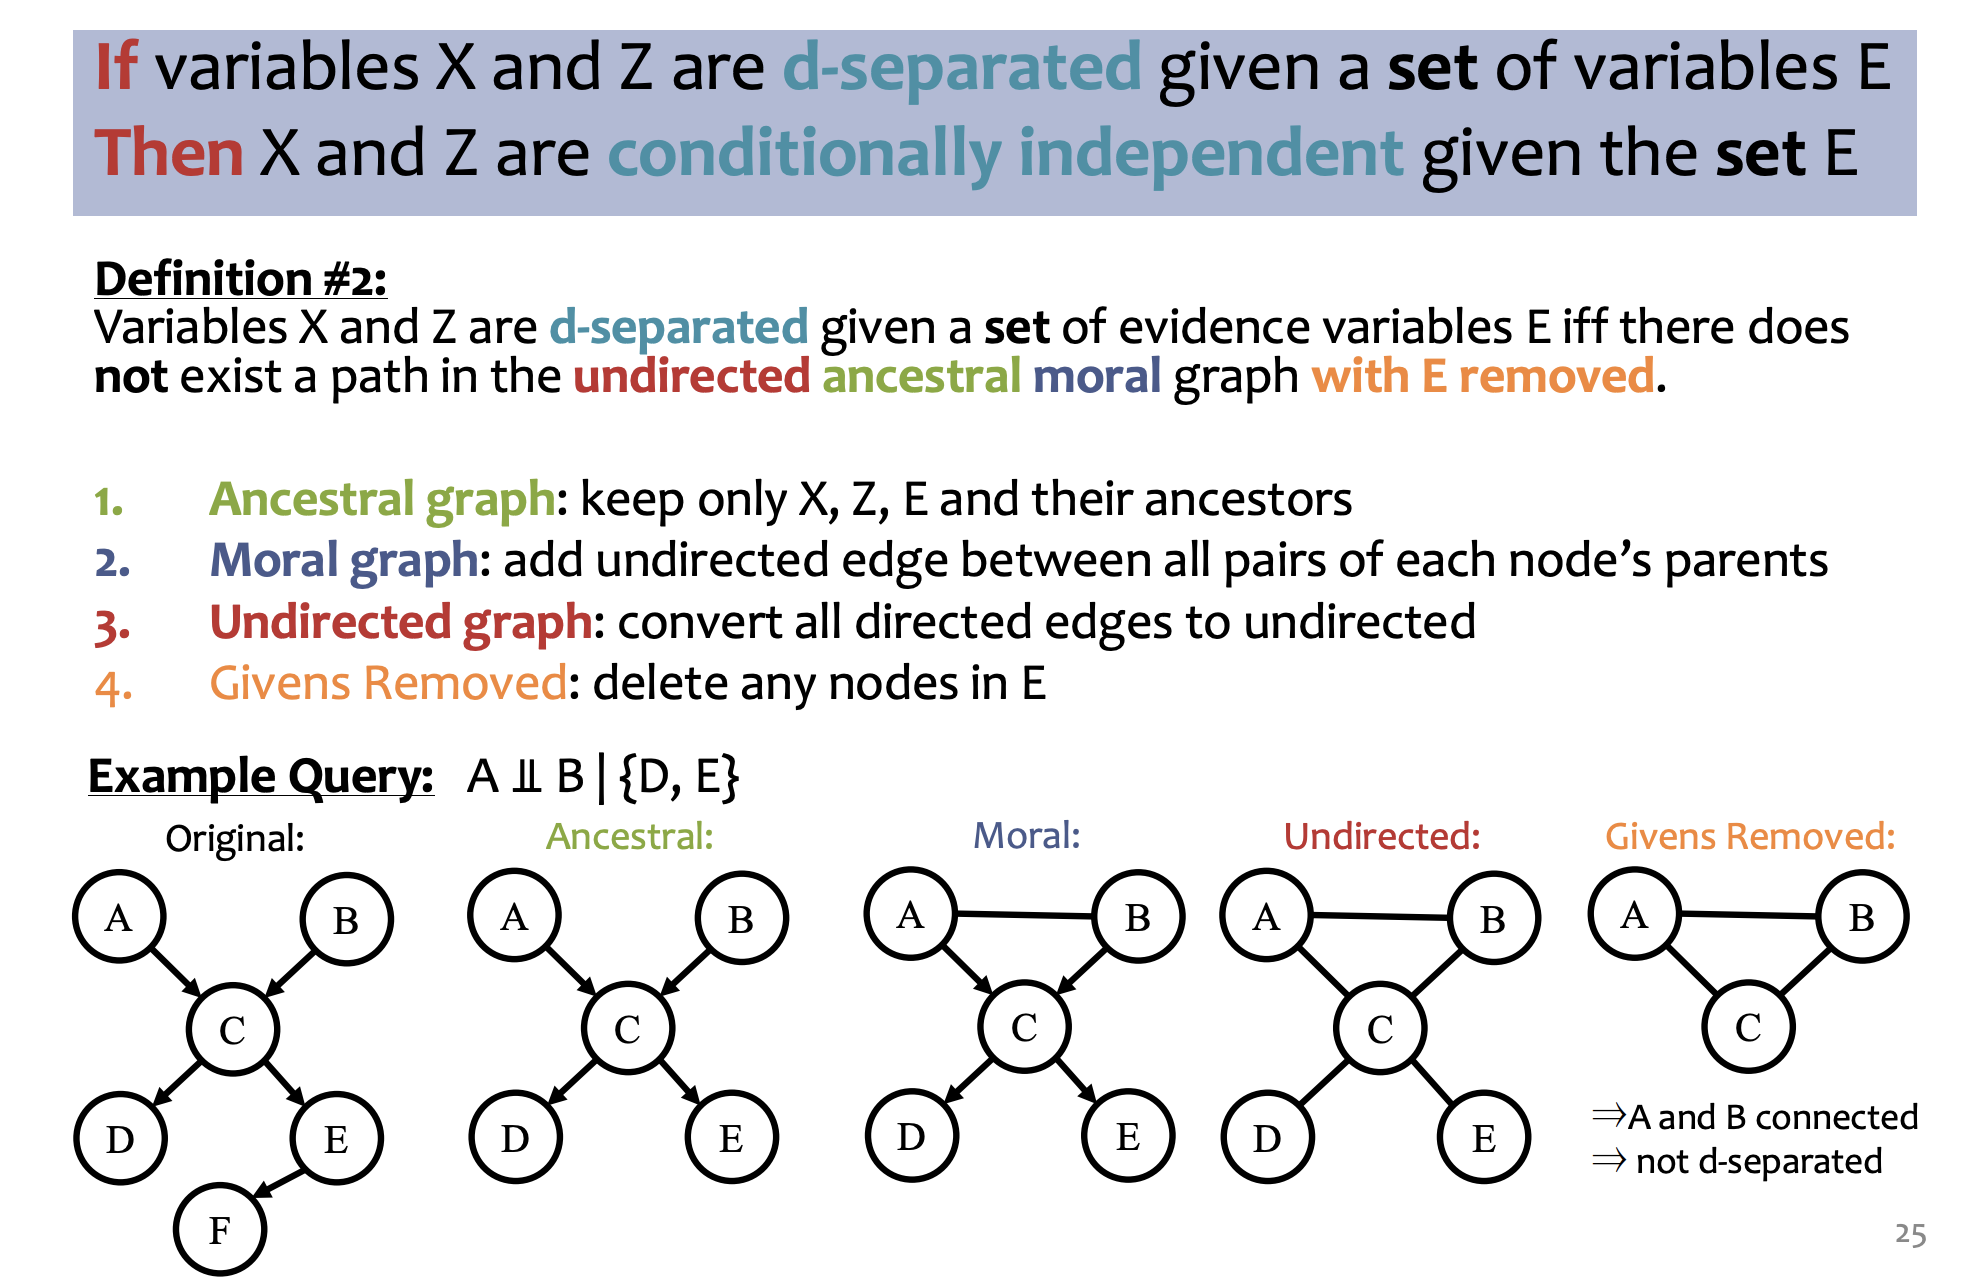
\includegraphics[width=\textwidth]{images/d-separation}
%\caption{ \tiny Image Credit: Matt Gormley (CMU).}
%\label{fig:d_separation}
\end{figure} 
\vfill
\tiny \hfill Image Credit: Matt Gormley (CMU). 
 \end{frame}
 
 
\begin{frame}{Worksheet for practice}
\end{frame}

\justfor{students}{
\begin{frame}{Revisiting the HMM statement}
\begin{quote}
The future is independent of the past given the current state
\end{quote}

Is this true? \\

\begin{enumerate}
\item   $Y_2 \indep Y_1 \cond X_2$ ?  \tiny(Try it.)  \normalsize \pause \redx \pause
\item  $Y_2 \indep Y_1 \cond X_2, \theta, \pi$ ?  \pause \greencheck \pause
\item (In fact,  $Y_2 \indep Y_1 \cond X_2, \theta$)
\end{enumerate}
\end{frame}
}

\begin{frame}{Fundamental property of Bayes networks}
Let us generalize this finding. \\

An oft-stated fact is:
\[ \textit{A node is independent of its non-descendants given its parents. } \]

\pause \tiny (Look again at the HMM)  \normalsize \pause 

This can easily be proven via d-separation.  
\begin{itemize}
\item The first step (``ancestral graph") will remove all of $X$'s children.
\item The fourth step (``remove givens") will remove $X$'s parents. 
\item Thus, $X$ will be disconnected from the rest of the graph.
\end{itemize}
\end{frame}


\begin{frame}{Markov blankets}
\begin{figure}[H]
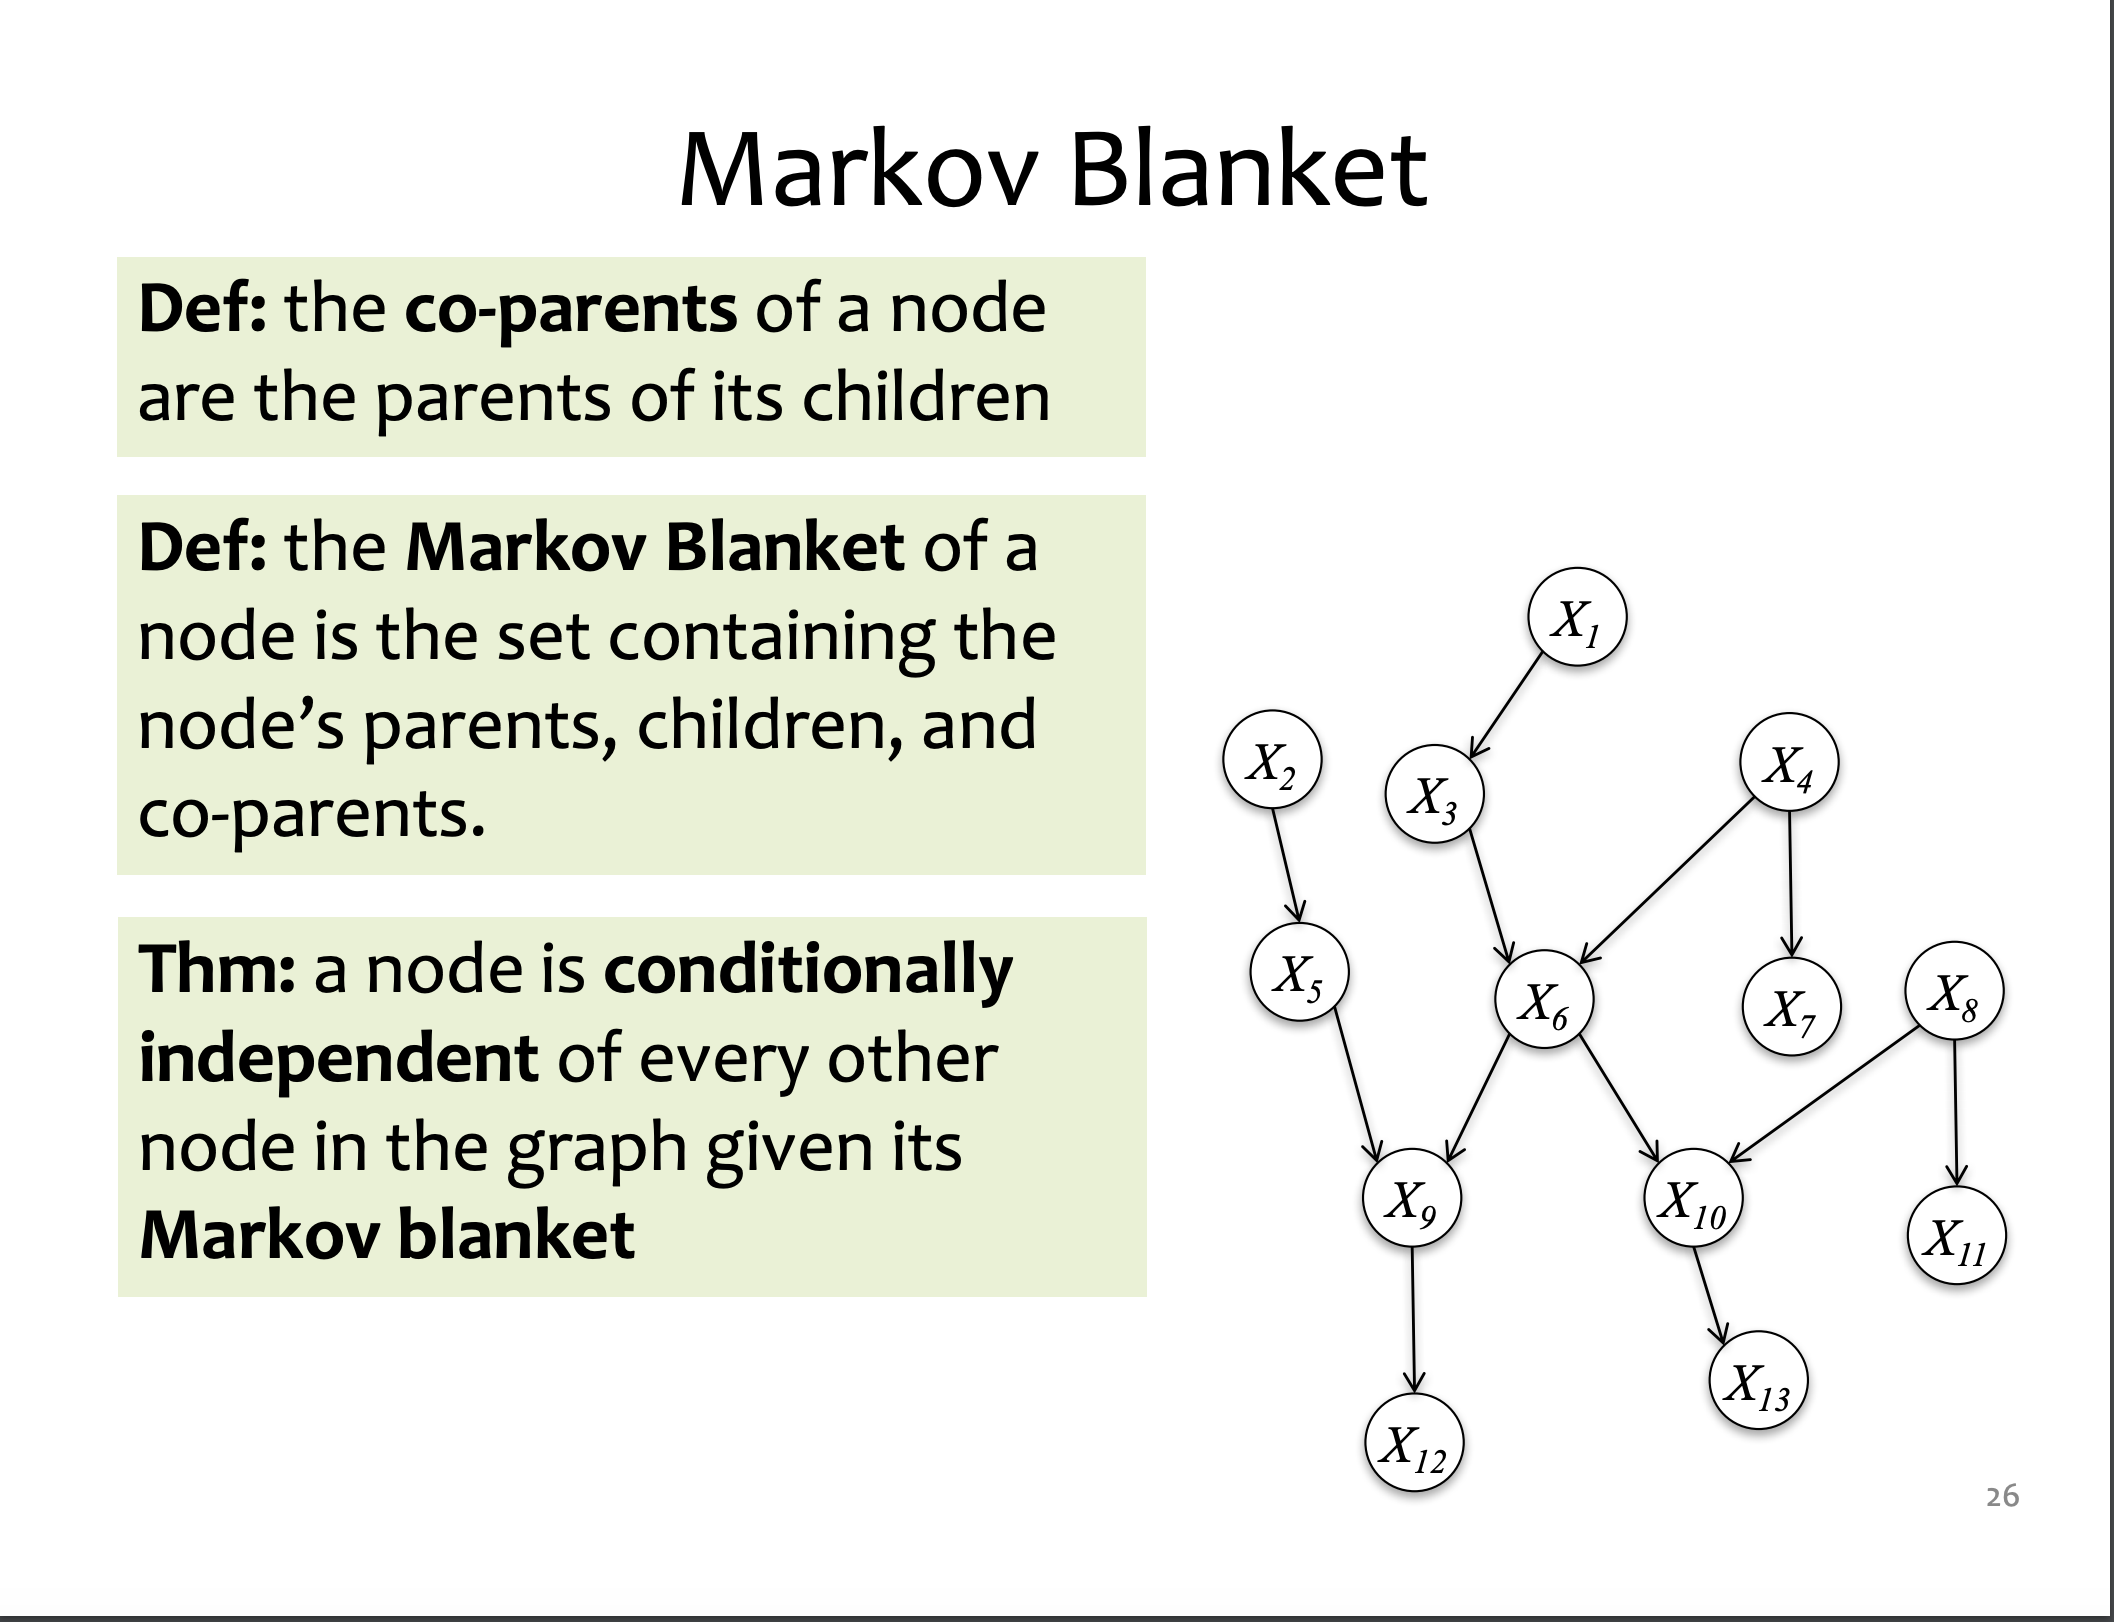
\includegraphics[width=.8\textwidth]{images/markov_blanket_1}
%\caption{ \tiny Image Credit: Matt Gormley (CMU).}
%\label{fig:d_separation}
\end{figure} 
\vfill
\tiny \hfill Image Credit: Matt Gormley (CMU).  \\
\pause 
\tiny \bf{Q}: What is the Markov Blanket of $X_6$?  Why?
 \end{frame}


\begin{frame}{Markov blankets}
\begin{figure}[H]
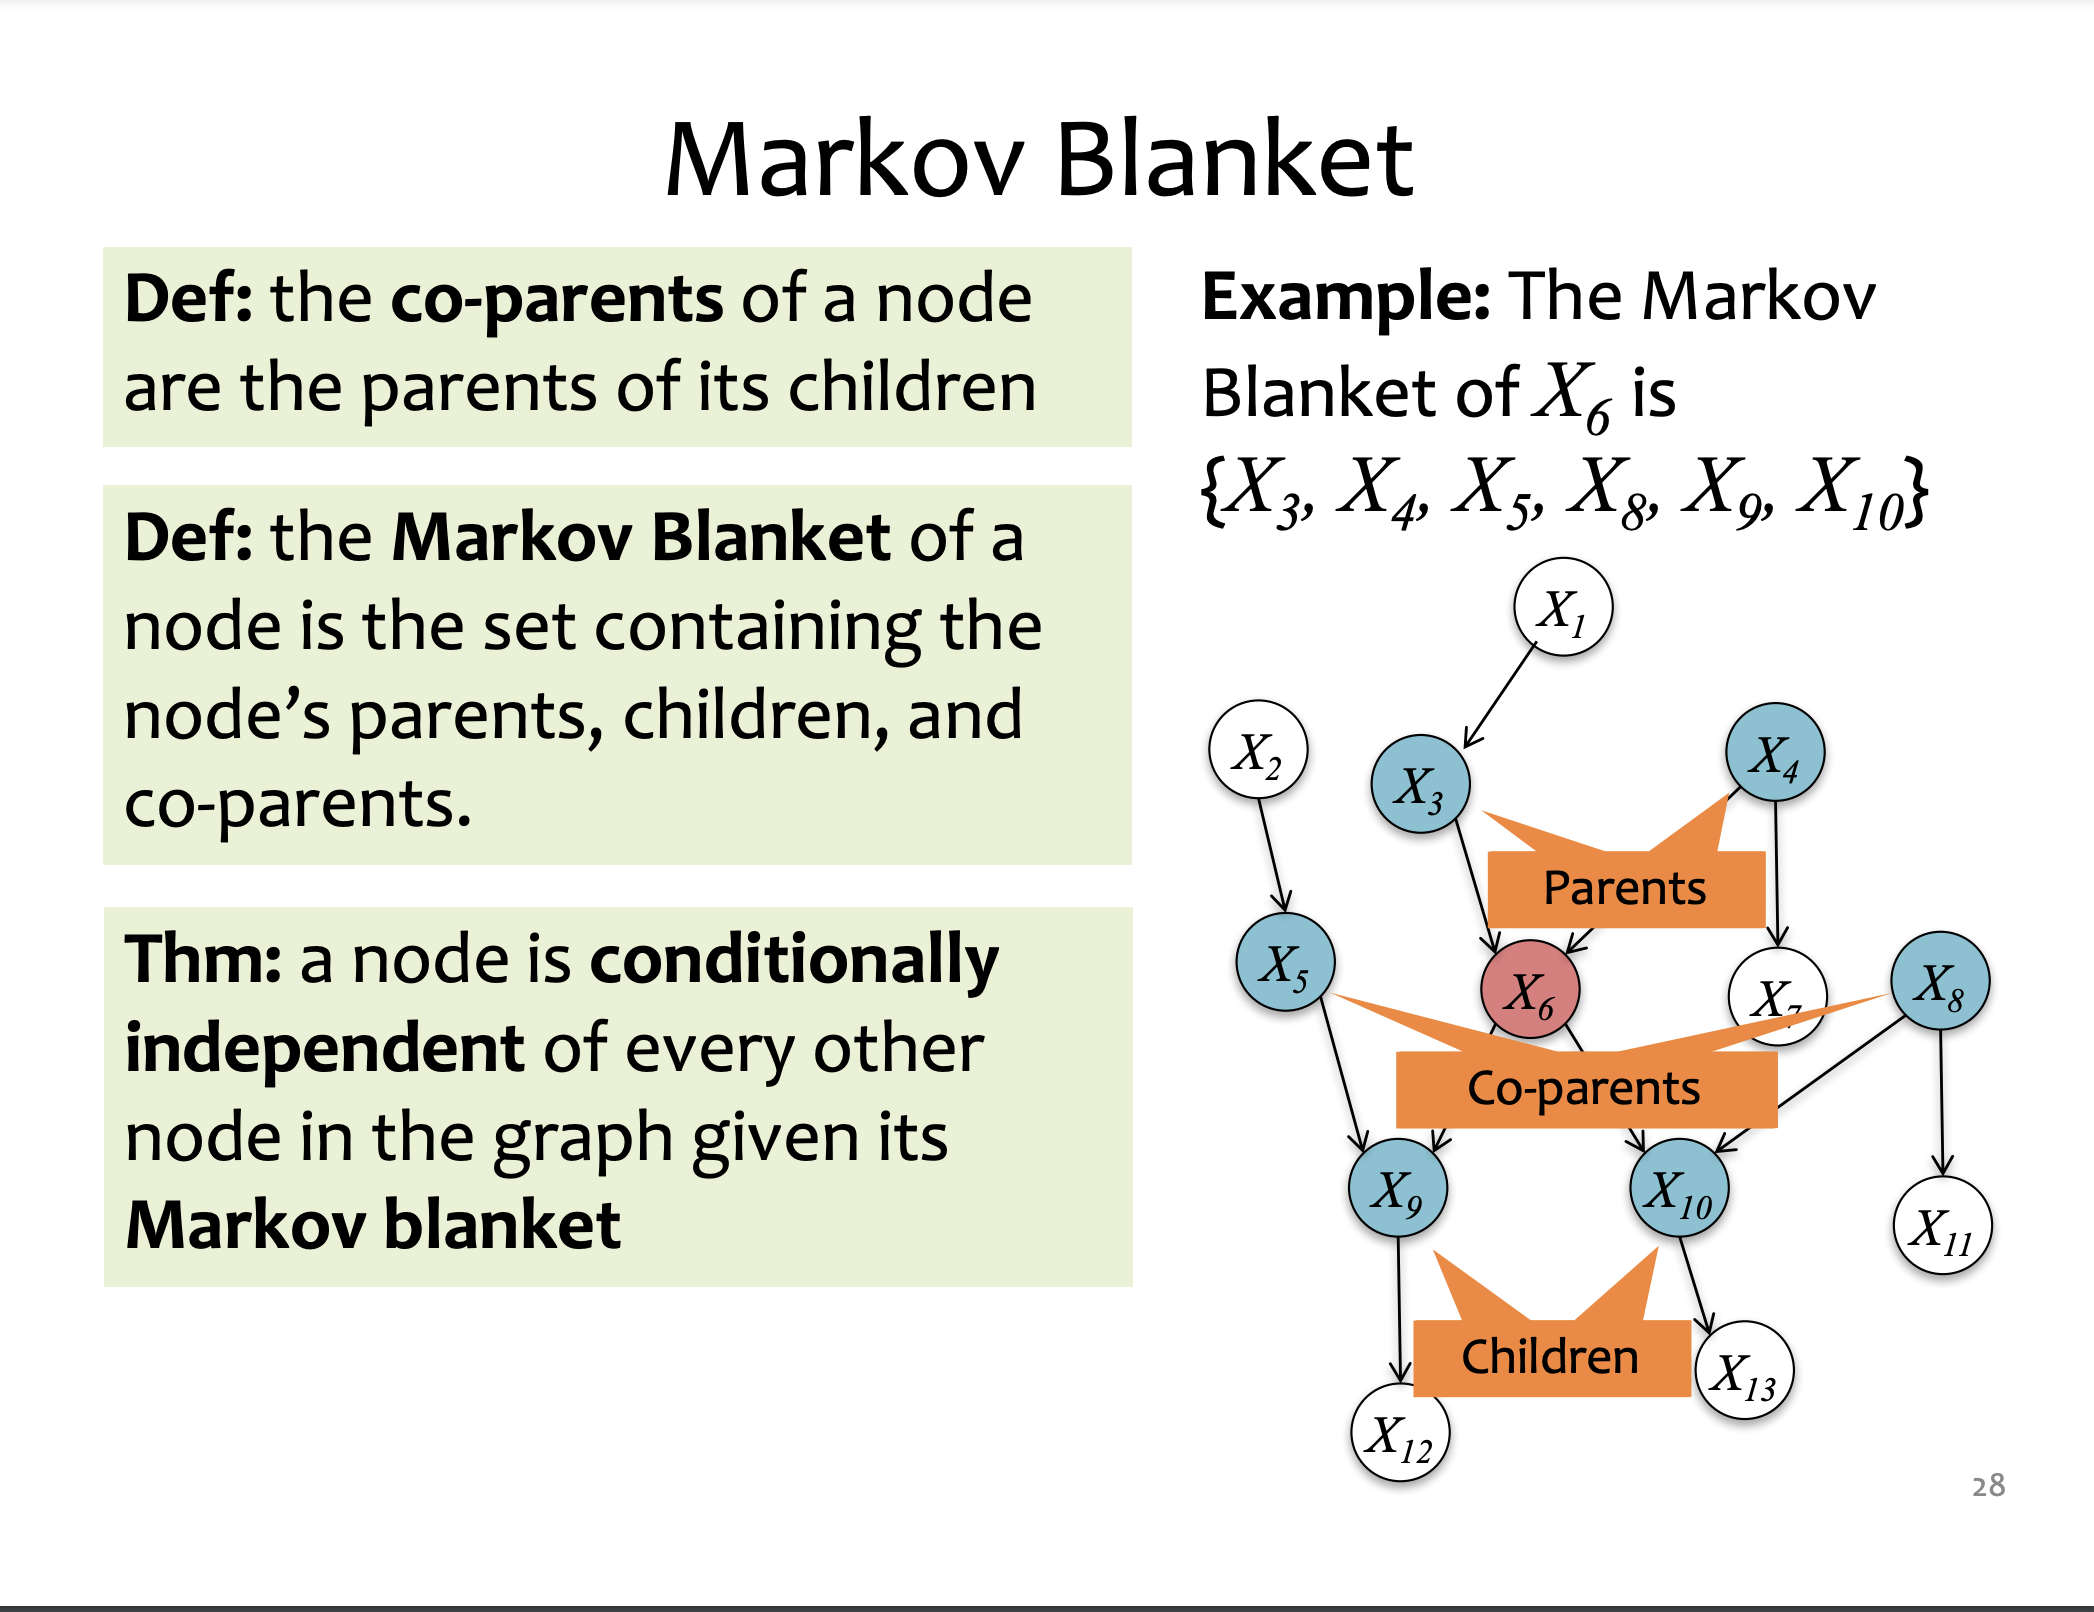
\includegraphics[width=.8\textwidth]{images/markov_blanket_2}
%\caption{ \tiny Image Credit: Matt Gormley (CMU).}
%\label{fig:d_separation}
\end{figure} 
\vfill
\tiny \hfill Image Credit: Matt Gormley (CMU). 
 \end{frame}

\begin{frame}{Markov Blankets: Why \textit{co}-parents?}

Why is it not sufficient for the Markov Blanket to only include the parents and children of $X_i$? \\
\pause
\vfill
The phenomenon of \alert{explaining away} means that the observations of child nodes will not block paths to the co-parents. \pause  \\
\vfill
This is why step 2 of the d-separation algorithm ("moralization") connects parents. \\
\vfill
In the previous graph, the transformed graph would still have paths from $X_6$ to, for example, $X_8$ (and to $X_{11}$).
\end{frame}

\begin{frame}{Proof of Markov Blanket statement}
Let us consider the conditional distribution of some variable $X_i$ given the factorization in \eqref{eqn:joint_factorization}:

\begin{align*}
 p(X_i  \cond X_{-i}) &= \df{ p(X_1, ..., X_n)}{ \ds\int  p(X_1, ..., X_n) d\, X_i} \\
 &= \df{\ds\prod_{k=1}^n p(X_k \cond \pi_k)}{\ds\int \ds\prod_{k=1}^n p(X_k \cond \pi_k) \; d\,X_i }
 \end{align*}
 
All terms will cancel in the numerator and denominator except for terms of the form
\begin{enumerate}
\item $p(X_i \cond \pi_i)$, i.e. terms where $i$ is the node itself
\item $\{p(X_k \cond \pi_k) : i \in \pi_k \} $, i.e. terms where $i$ is one of the parents.
\end{enumerate}

Terms of type (1) will depend on $X_i$'s parents, and terms of type (2) will depend on $X_i$'s children and co-parents.

\end{frame}
 

\end{document}